% Options for packages loaded elsewhere
\PassOptionsToPackage{unicode}{hyperref}
\PassOptionsToPackage{hyphens}{url}
%
\documentclass[
]{article}
\usepackage{amsmath,amssymb}
\usepackage{lmodern}
\usepackage{iftex}
\ifPDFTeX
  \usepackage[T1]{fontenc}
  \usepackage[utf8]{inputenc}
  \usepackage{textcomp} % provide euro and other symbols
\else % if luatex or xetex
  \usepackage{unicode-math}
  \defaultfontfeatures{Scale=MatchLowercase}
  \defaultfontfeatures[\rmfamily]{Ligatures=TeX,Scale=1}
\fi
% Use upquote if available, for straight quotes in verbatim environments
\IfFileExists{upquote.sty}{\usepackage{upquote}}{}
\IfFileExists{microtype.sty}{% use microtype if available
  \usepackage[]{microtype}
  \UseMicrotypeSet[protrusion]{basicmath} % disable protrusion for tt fonts
}{}
\makeatletter
\@ifundefined{KOMAClassName}{% if non-KOMA class
  \IfFileExists{parskip.sty}{%
    \usepackage{parskip}
  }{% else
    \setlength{\parindent}{0pt}
    \setlength{\parskip}{6pt plus 2pt minus 1pt}}
}{% if KOMA class
  \KOMAoptions{parskip=half}}
\makeatother
\usepackage{xcolor}
\IfFileExists{xurl.sty}{\usepackage{xurl}}{} % add URL line breaks if available
\IfFileExists{bookmark.sty}{\usepackage{bookmark}}{\usepackage{hyperref}}
\hypersetup{
  pdftitle={RandomData Revenue Administration Primer},
  hidelinks,
  pdfcreator={LaTeX via pandoc}}
\urlstyle{same} % disable monospaced font for URLs
\usepackage[margin=1in]{geometry}
\usepackage{graphicx}
\makeatletter
\def\maxwidth{\ifdim\Gin@nat@width>\linewidth\linewidth\else\Gin@nat@width\fi}
\def\maxheight{\ifdim\Gin@nat@height>\textheight\textheight\else\Gin@nat@height\fi}
\makeatother
% Scale images if necessary, so that they will not overflow the page
% margins by default, and it is still possible to overwrite the defaults
% using explicit options in \includegraphics[width, height, ...]{}
\setkeys{Gin}{width=\maxwidth,height=\maxheight,keepaspectratio}
% Set default figure placement to htbp
\makeatletter
\def\fps@figure{htbp}
\makeatother
\setlength{\emergencystretch}{3em} % prevent overfull lines
\providecommand{\tightlist}{%
  \setlength{\itemsep}{0pt}\setlength{\parskip}{0pt}}
\setcounter{secnumdepth}{5}
\usepackage{booktabs}
\usepackage{longtable}
\usepackage{array}
\usepackage{multirow}
\usepackage{wrapfig}
\usepackage{float}
\usepackage{colortbl}
\usepackage{pdflscape}
\usepackage{tabu}
\usepackage{threeparttable}
\usepackage[normalem]{ulem}
\PassOptionsToPackage{table}{xcolor}
\ifLuaTeX
  \usepackage{selnolig}  % disable illegal ligatures
\fi

\title{RandomData Revenue Administration Primer}
\author{}
\date{\vspace{-2.5em}}

\begin{document}
\maketitle

{
\setcounter{tocdepth}{2}
\tableofcontents
}
\newpage

\hypertarget{cover}{%
\section{Cover}\label{cover}}

This is a dummy version of a reporting system in R I made. This version
to share the code.

None of the data is real, it is all randomly generated.

\hypertarget{notes-on-data}{%
\subsection{Notes on Data}\label{notes-on-data}}

This section aims to list resources that staff can find additional
resources for research.

Additional internal resources for data:

\begin{itemize}
\item
  \href{}{-}
\item
  \href{}{-}
\item
  \href{}{-}
\item
  \href{}{-}
\item
  \href{}{-}
\end{itemize}

External Sources:

\begin{itemize}
\item
  \href{https://idea.usaid.gov/cd/albania/}{Country Macro-Overview
  Dashboard}
\item
  \href{https://wits.worldbank.org/Default.aspx?lang=en}{World
  Integrated Trade Solution} Website for world trade and tariff data
  visualizations
\item
  \href{https://live.sixfold.com/}{EUR Truck and Sea Crossing Time
  Map}\\
  Only free during COVID
\item
  \href{https://comtrade.un.org/Data/Doc/api/ex/r}{NowCast Trade API}
\end{itemize}

\newpage

\hypertarget{national-accounts}{%
\section{National Accounts}\label{national-accounts}}

\hypertarget{national-accounts---output}{%
\subsection{National Accounts -
Output}\label{national-accounts---output}}

\begin{center}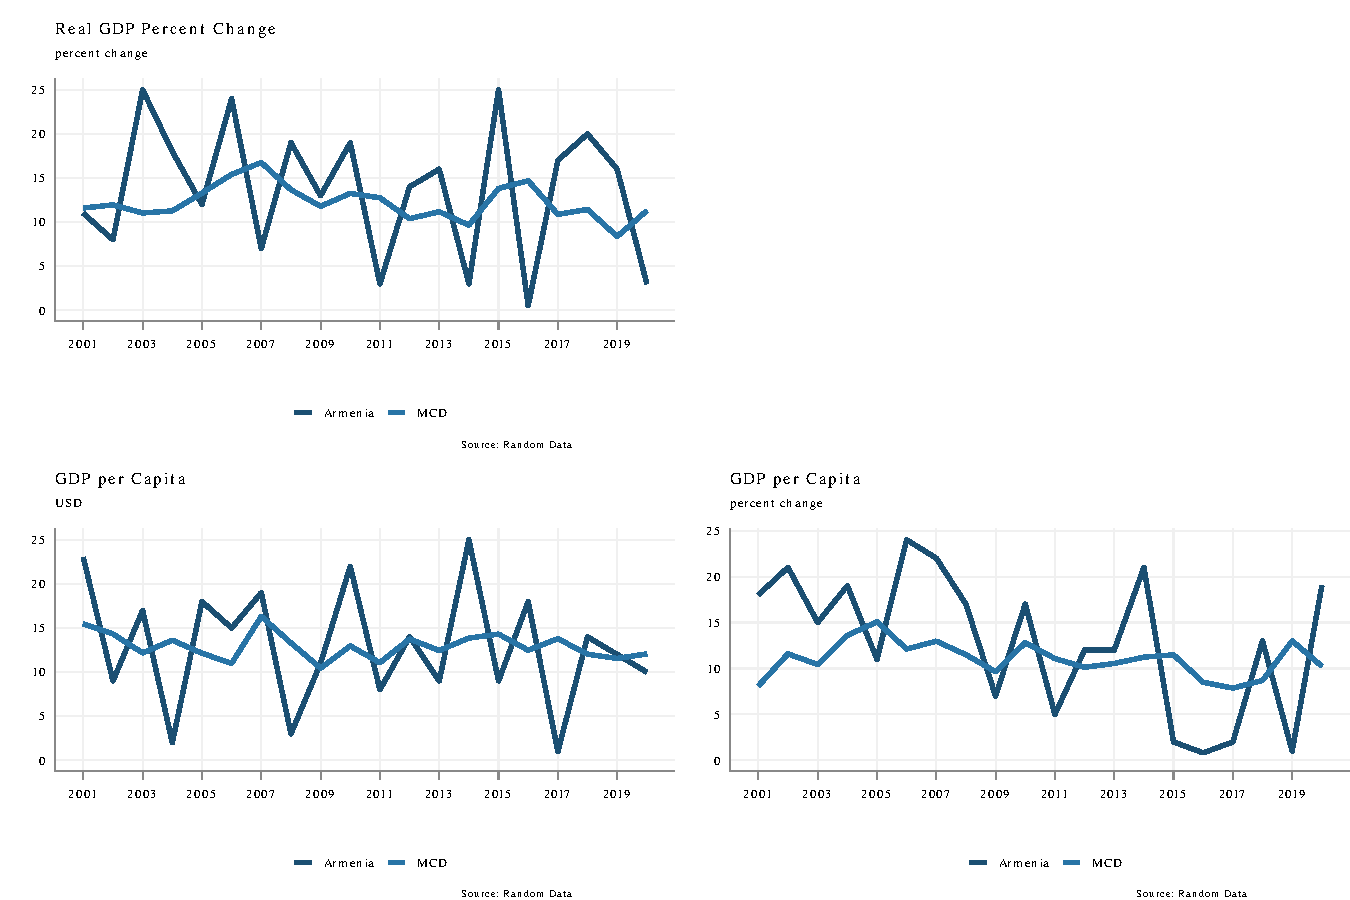
\includegraphics{RandomData_MCD__files/figure-latex/ouput-1} \end{center}
\newpage

\hypertarget{national-accounts---demand}{%
\subsection{National Accounts -
Demand}\label{national-accounts---demand}}

\begin{center}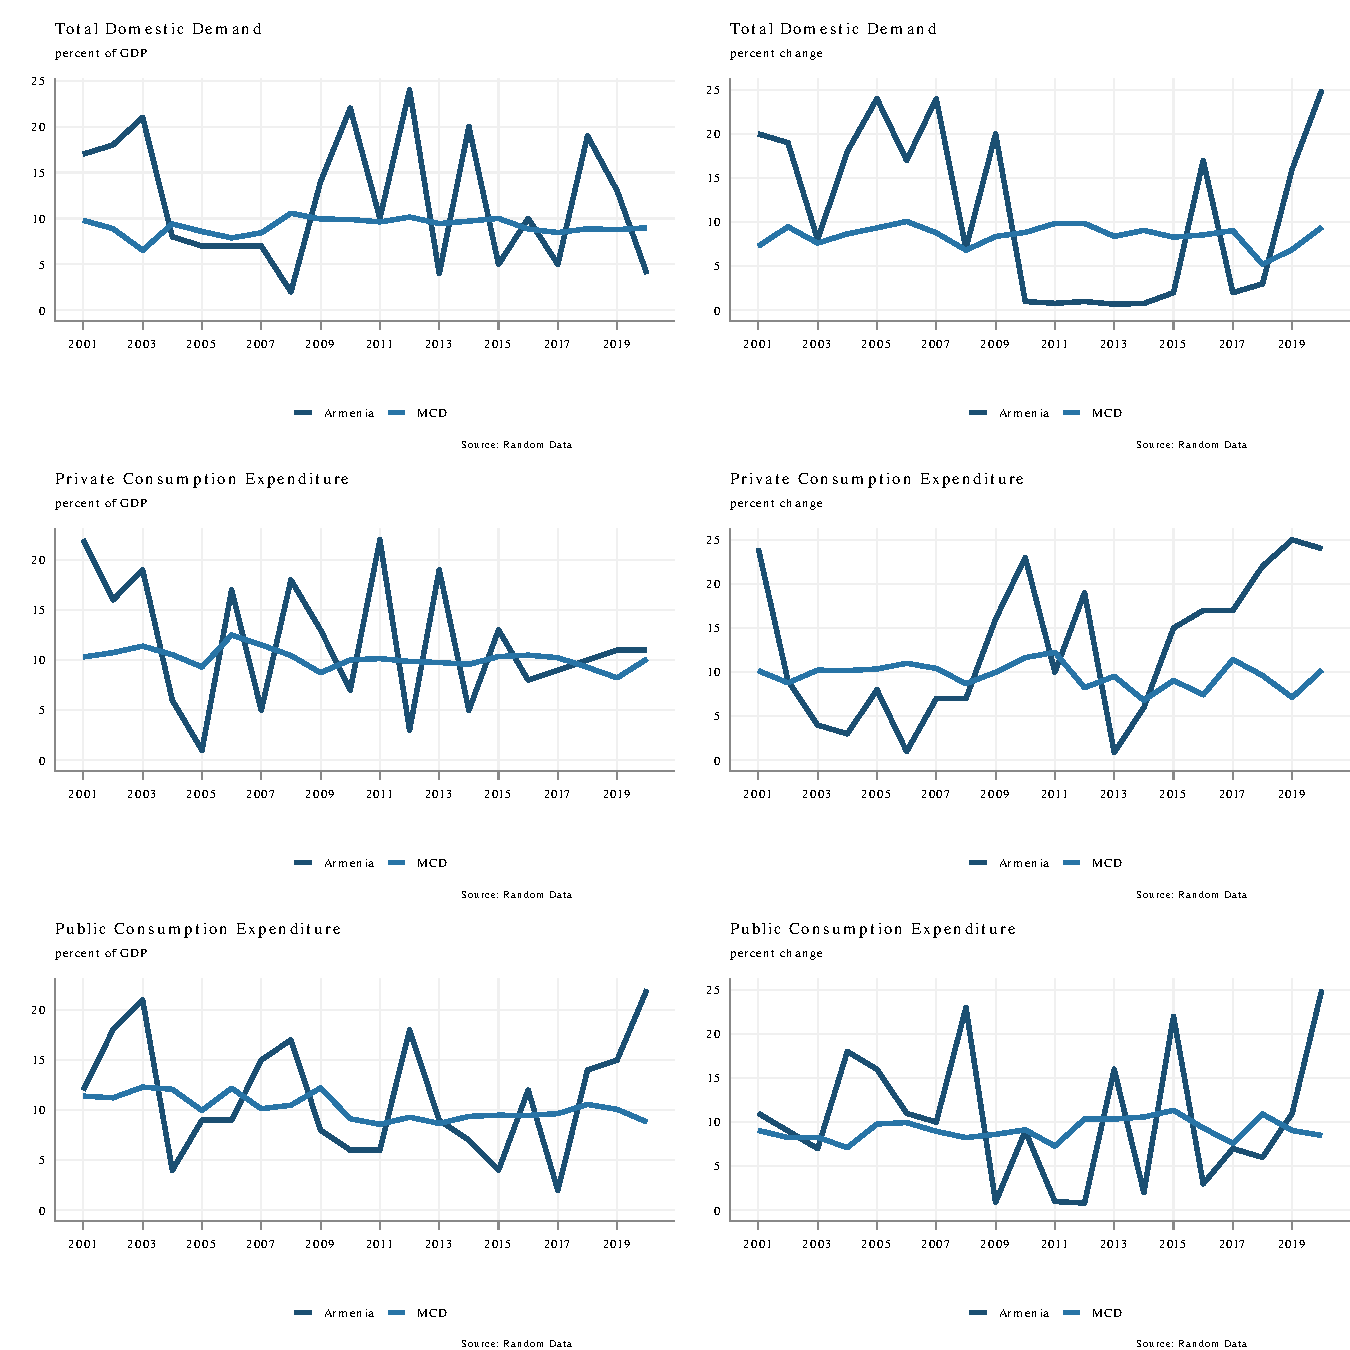
\includegraphics{RandomData_MCD__files/figure-latex/demand-1} \end{center}
\newpage

\hypertarget{national-accounts---trade}{%
\subsection{National Accounts - Trade}\label{national-accounts---trade}}

\begin{center}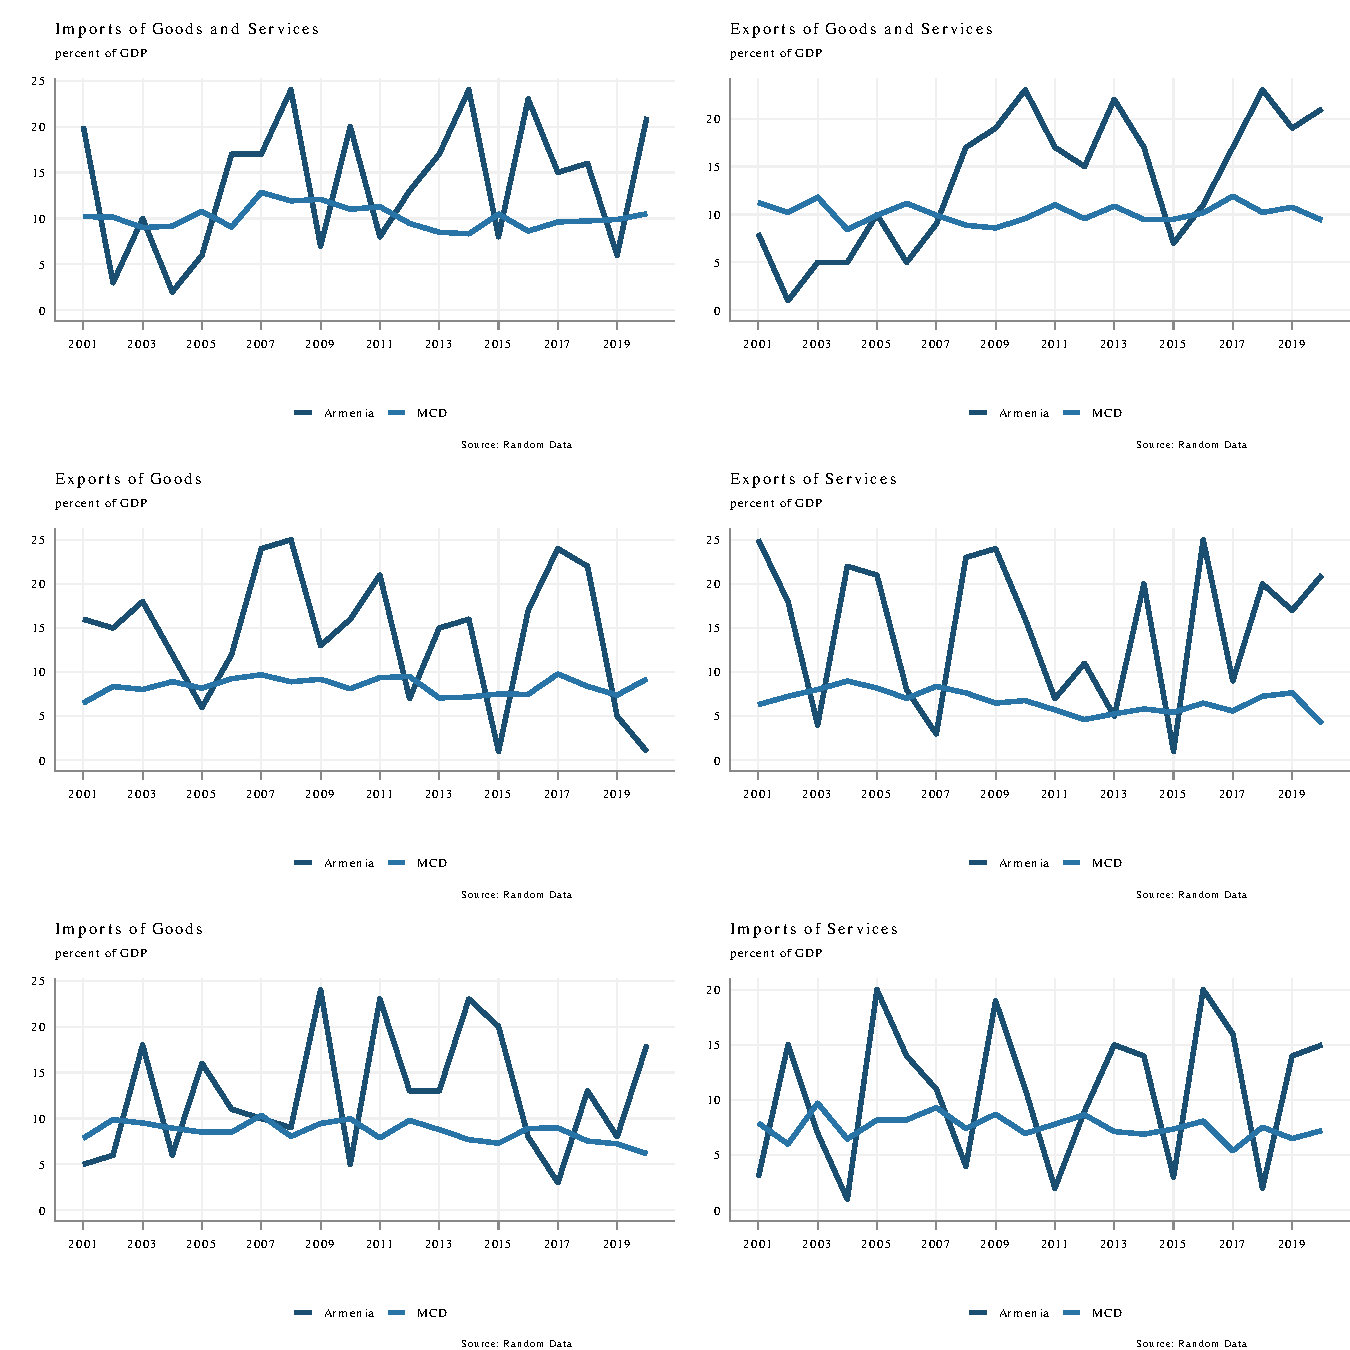
\includegraphics{RandomData_MCD__files/figure-latex/trade-1} \end{center}
\newpage

\hypertarget{revenue-data}{%
\section{Revenue Data}\label{revenue-data}}

\hypertarget{general-government-revenue-overview}{%
\subsection{General Government Revenue
Overview}\label{general-government-revenue-overview}}

\begin{center}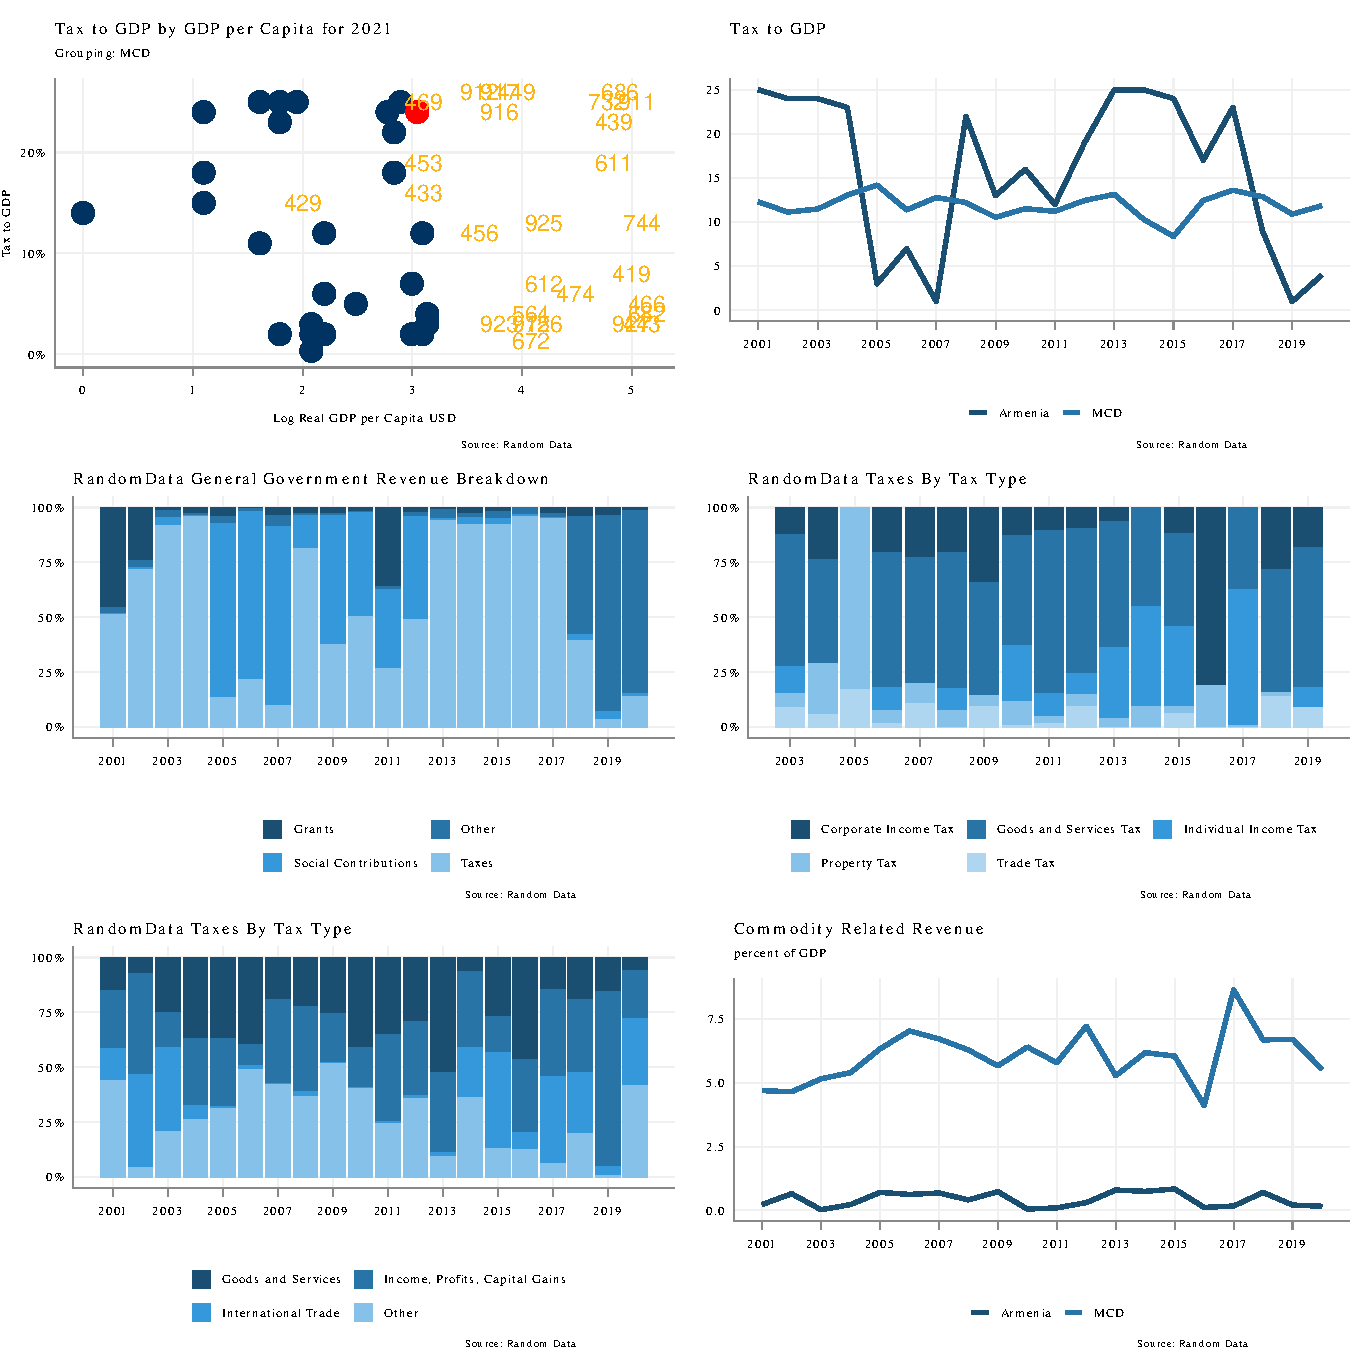
\includegraphics{RandomData_MCD__files/figure-latex/01_scatter_WEO_WoRLD_TaxGDP_to_GDPPC-1} \end{center}
\newpage

\hypertarget{revenue-data---direct-taxes}{%
\subsection{Revenue Data - Direct
Taxes}\label{revenue-data---direct-taxes}}

\hypertarget{revenue-data---direct-taxes---cit}{%
\subsubsection{Revenue Data - Direct Taxes -
CIT}\label{revenue-data---direct-taxes---cit}}

\begin{center}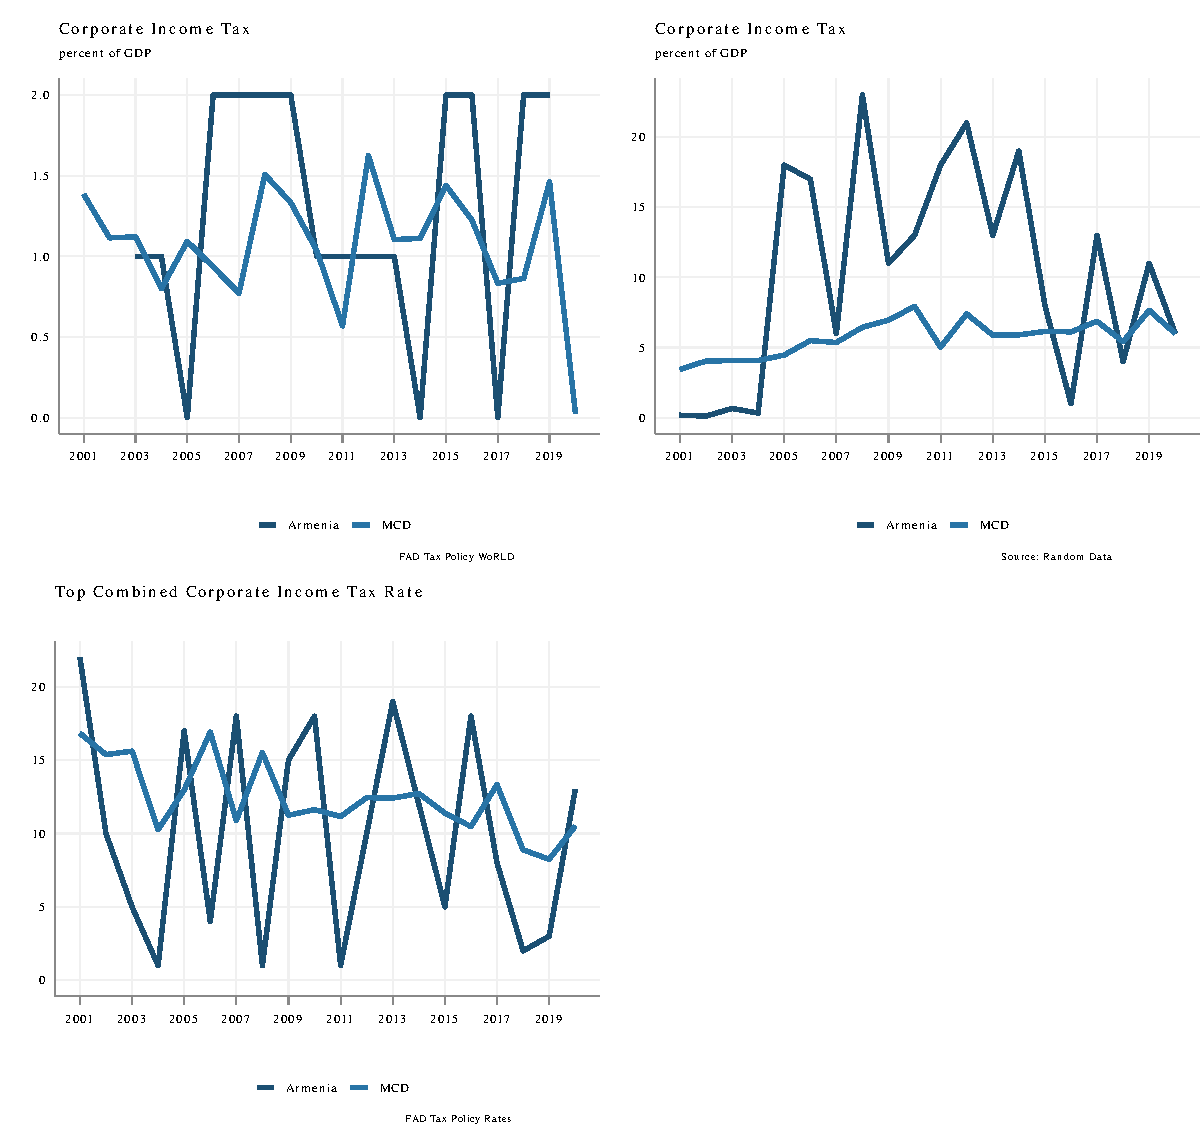
\includegraphics{RandomData_MCD__files/figure-latex/weoDirectTaxesCorporate-1} \end{center}

\newpage

\hypertarget{revenue-data---direct-taxes---cit---bvd-orbis-firm-level-financial-data}{%
\paragraph{Revenue Data - Direct Taxes - CIT - BvD Orbis Firm Level
Financial
Data}\label{revenue-data---direct-taxes---cit---bvd-orbis-firm-level-financial-data}}

removed

\newpage

\hypertarget{revenue-data---direct-taxes---cit---orbis-risk-differentiation-framework}{%
\paragraph{Revenue Data - Direct Taxes - CIT - Orbis Risk
Differentiation
Framework}\label{revenue-data---direct-taxes---cit---orbis-risk-differentiation-framework}}

removed

\newpage

\hypertarget{revenue-data---direct-taxes---individual-income-tax}{%
\subsubsection{Revenue Data - Direct Taxes - Individual Income
Tax}\label{revenue-data---direct-taxes---individual-income-tax}}

\begin{center}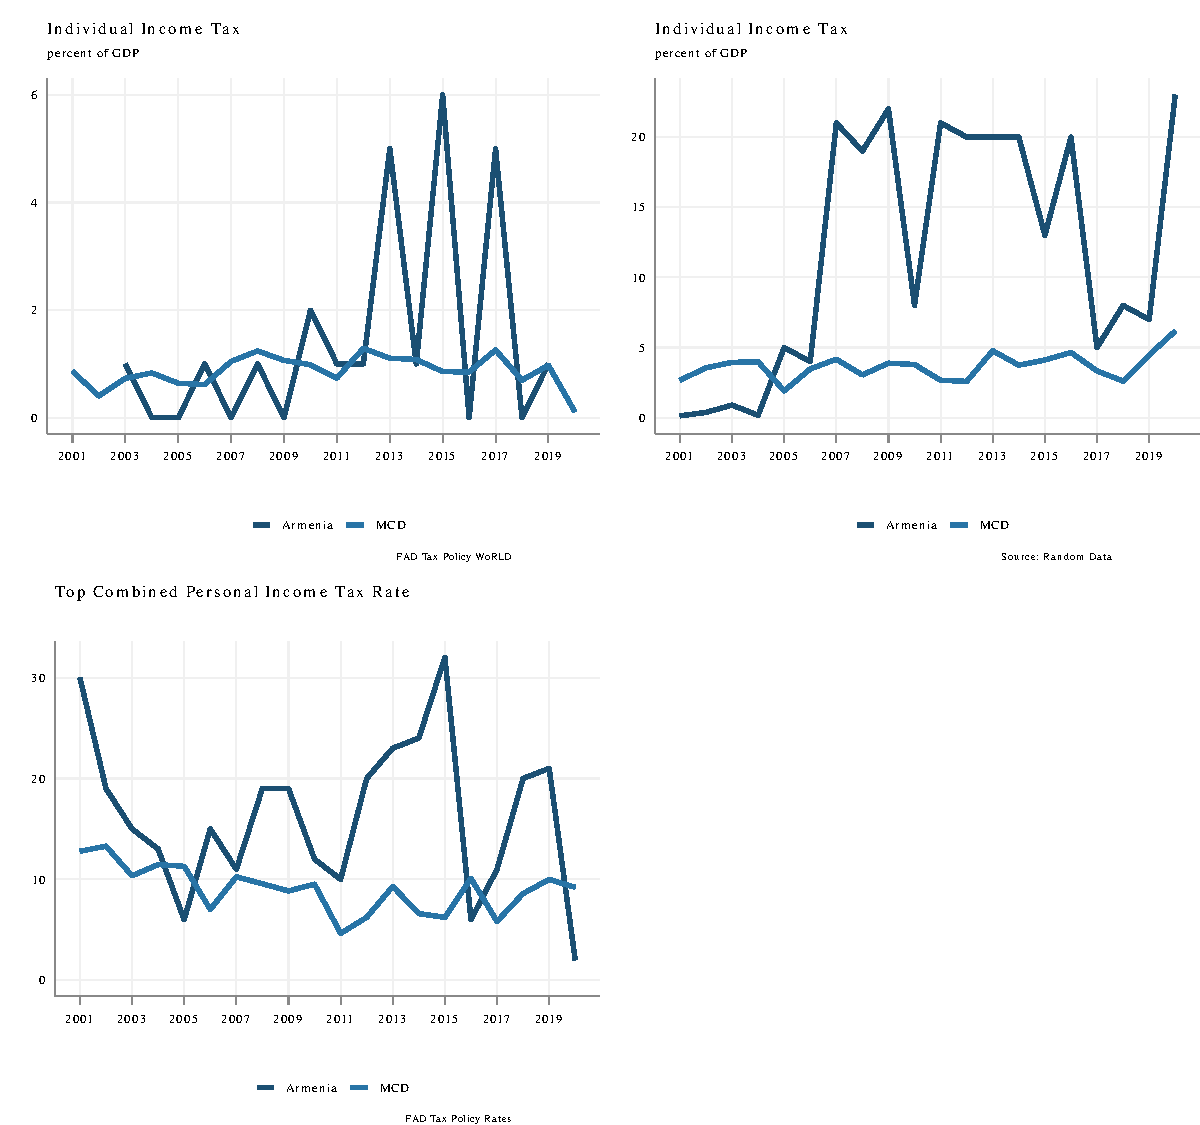
\includegraphics{RandomData_MCD__files/figure-latex/weoDirectTaxesIndividual-1} \end{center}

\newpage

\hypertarget{revenue-data---indirect-taxes}{%
\subsection{Revenue Data - Indirect
Taxes}\label{revenue-data---indirect-taxes}}

\begin{center}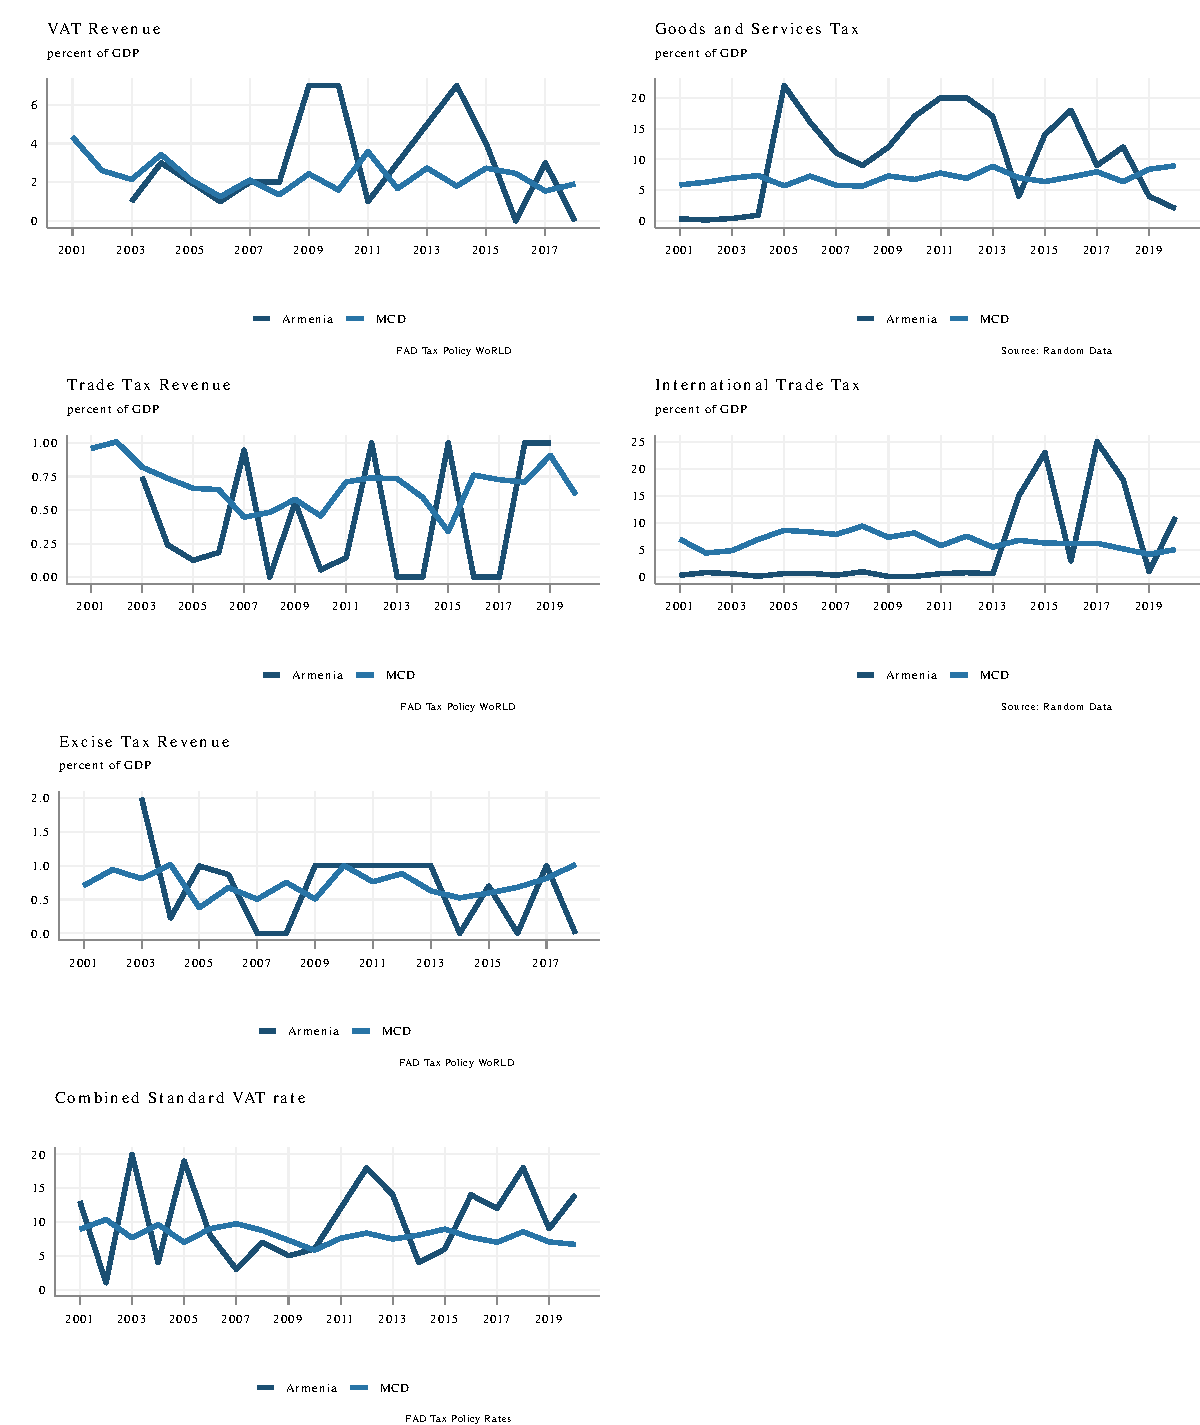
\includegraphics{RandomData_MCD__files/figure-latex/weoInDirectTaxesLine-1} \end{center}

\newpage

\hypertarget{international-survey-on-revenue-administrations-isora}{%
\section{International Survey on Revenue Administrations
(ISORA)}\label{international-survey-on-revenue-administrations-isora}}

The IMF has collaboratively developed this survey along with the
Inter-American Center of Tax Administrations (CIAT), the Intra-European
Organisation of Tax Administrations (IOTA), and the Organisation for
Economic Cooperation and Development (OECD).

Accordingly, it is the IMF's vision to:

\begin{itemize}
\tightlist
\item
  Assist revenue administrations globally to improve their focus
  performance measurement and reporting
\item
  Provide a larger set of revenue administration data to improve advice
  and analysis
\item
  Develop data and analyses that can improve cross-country comparisons
\end{itemize}

Provided Links:

\begin{itemize}
\tightlist
\item
  \href{https://data.rafit.org/}{ISORA Website}
\end{itemize}

\hypertarget{return-filing}{%
\subsection{Return Filing}\label{return-filing}}

removed

\newpage

\hypertarget{human-resources}{%
\subsection{Human Resources}\label{human-resources}}

removed

\newpage

\hypertarget{fiscal-position}{%
\section{Fiscal Position}\label{fiscal-position}}

\begin{center}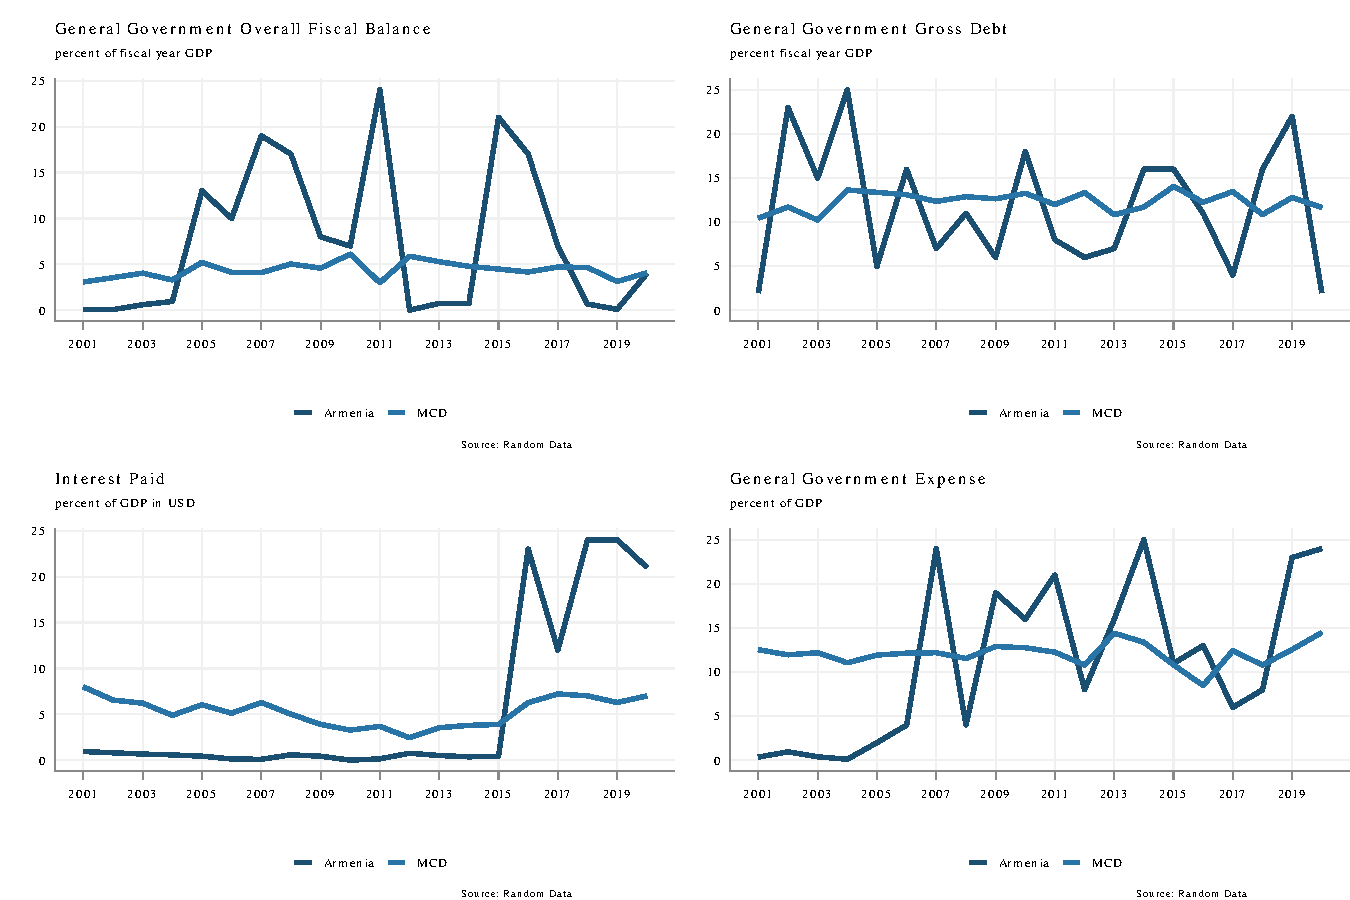
\includegraphics{RandomData_MCD__files/figure-latex/fiscal_position-1} \end{center}

\hypertarget{duties}{%
\section{Duties}\label{duties}}

\hypertarget{duties---agricultural-duties}{%
\subsection{Duties - Agricultural
Duties}\label{duties---agricultural-duties}}

\begin{center}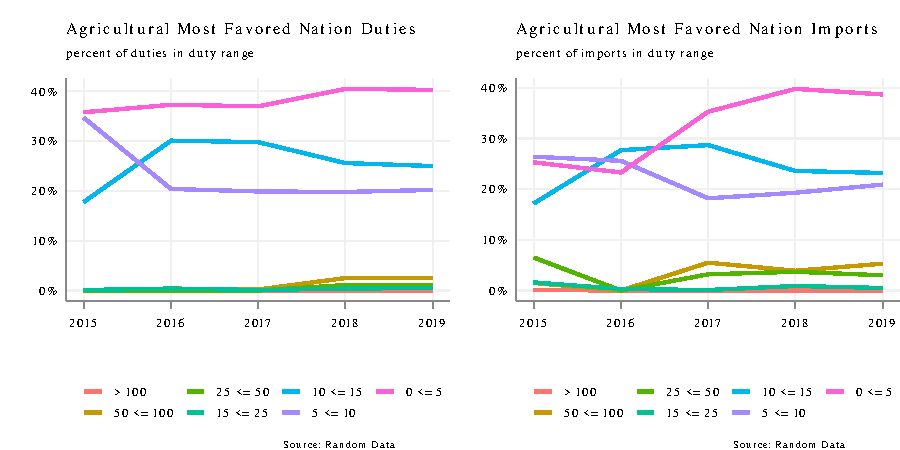
\includegraphics{RandomData_MCD__files/figure-latex/agricultureal_duties-1} \end{center}

\hypertarget{duties---non-agricultural-duties}{%
\subsection{Duties - Non-Agricultural
Duties}\label{duties---non-agricultural-duties}}

\begin{center}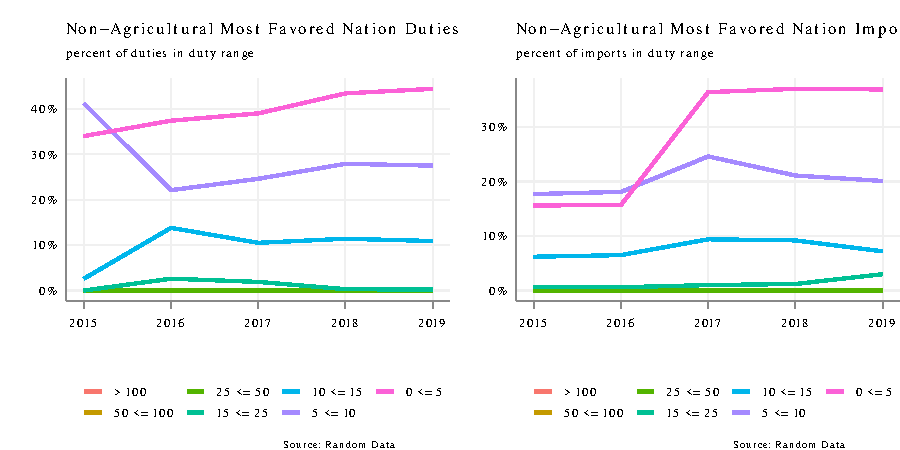
\includegraphics{RandomData_MCD__files/figure-latex/non-agricultureal_duties-1} \end{center}
\newpage

\hypertarget{duty-definitions}{%
\subsection{Duty Definitions}\label{duty-definitions}}

Bound tariffs are specific commitments made by individual WTO member
governments. The bound tariff is the maximum MFN tariff level for a
given commodity line. When countries join the WTO or when WTO members
negotiate tariff levels with each other during trade rounds, they make
agreements about bound tariff rates, rather than actually applied rates.

Bound tariffs are not necessarily the rate that a WTO member applies in
practice to other WTO members' products. Members have the flexibility
increase or decrease their tariffs (on a non-discriminatory basis) so
long as they didn't raise them above their bound levels. If one WTO
member raises applied tariffs above their bound level, other WTO members
can take the country to dispute settlement. If the country did not
reduced applied tariffs below their bound levels, other countries could
request compensation in the form of higher tariffs of their own. In
other words, the applied tariff is less than or equal to the bound
tariff in practice for any particular product.

The gap between the bound and applied MFN rates is called the binding
overhang. Trade economists argue that a large binding overhang makes a
country's trade policies less predictable. This gap tends to be small on
average in industrial countries and often fairly large in developing
countries.

\href{https://wits.worldbank.org/wits/wits/witshelp/content/data_retrieval/p/intro/c2.types_of_tariffs.htm}{Text
Citation World Bank}

Most Favoured Nation (MFN) tariffs are a tariff level that a member of
the General Agreement on Tariffs and Trade of the WTO charges on a good
to other members, i.e.~a country with a most favoured nation status (see
UNCTAD, 2018) It applies to imports from trading partners-members of the
World Trade Organization (WTO), unless the country has a preferential
trade agreement. It is the lowest possible tariff a country can assess
on another country.

\href{https://sdgpulse.unctad.org/glossary/mfn-tariffs/}{Text Cititation
UNCTAD}

\hypertarget{balance-of-payments}{%
\section{Balance of Payments}\label{balance-of-payments}}

\begin{center}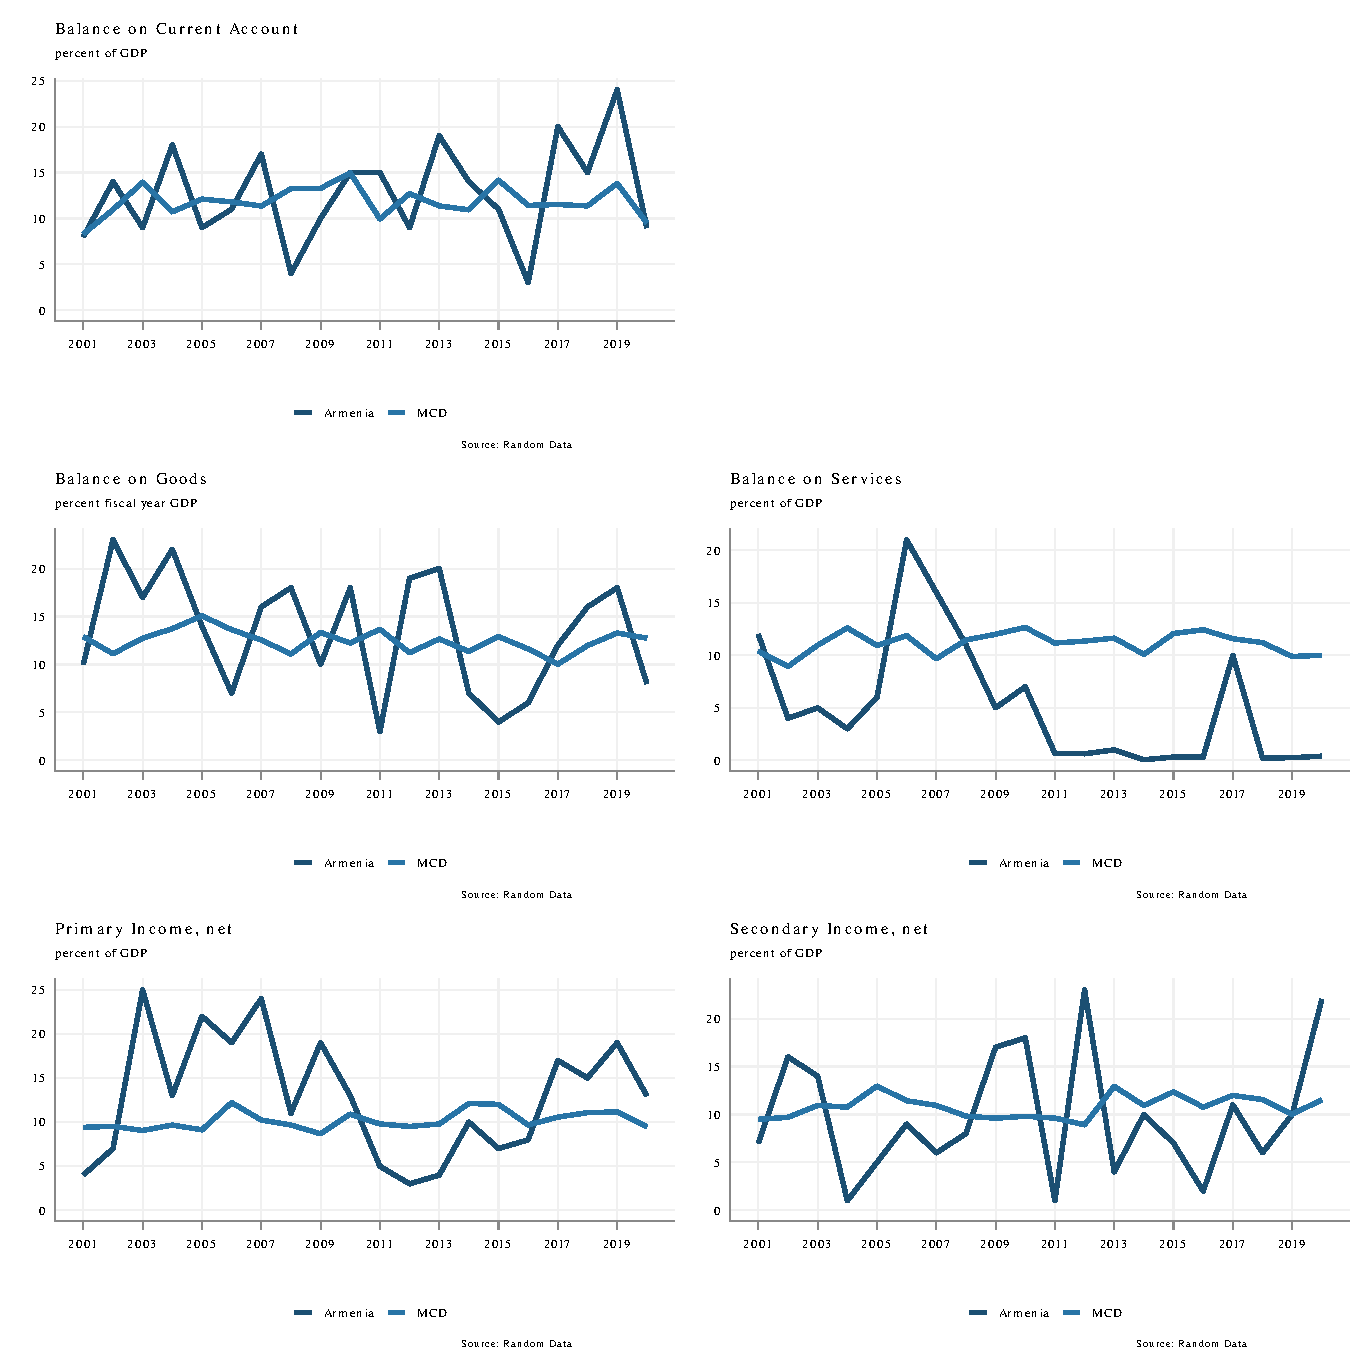
\includegraphics{RandomData_MCD__files/figure-latex/current_account-1} \end{center}

\newpage

\hypertarget{price-labor-and-monetary}{%
\section{Price, Labor, and Monetary}\label{price-labor-and-monetary}}

\begin{center}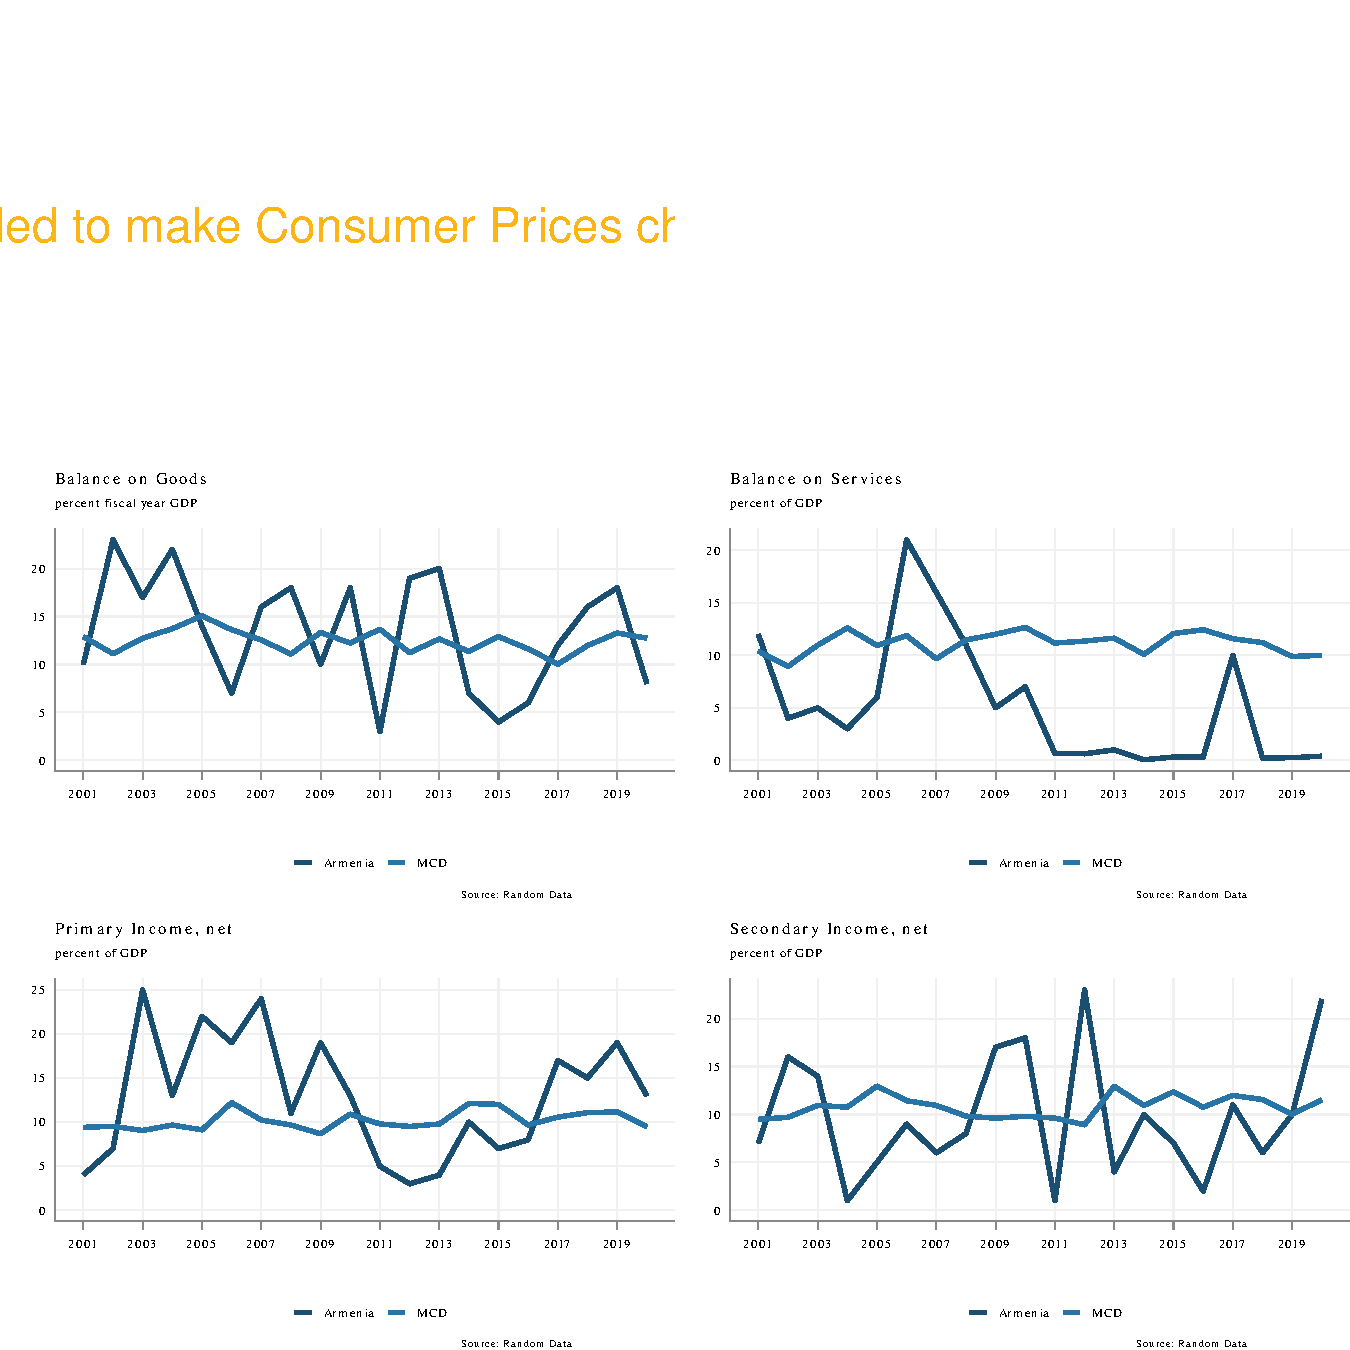
\includegraphics{RandomData_MCD__files/figure-latex/plm-1} \end{center}

\newpage

\hypertarget{appendix}{%
\section{Appendix}\label{appendix}}

removed

\end{document}
